%------------------------------------------------
% Latex-Grundgerüst für Seminarausarbeitungen
%
% zu Erzeugen mit
%   pdflatex ausarbeitung.tex
%
% von Carsten Gutwenger, Nils Kriege
% 
%------------------------------------------------

\documentclass[a4paper,12pt,twoside]{article}
\usepackage[a4paper,left=3.5cm,right=2.5cm,bottom=3.5cm,top=3cm]{geometry}

% Encoding der .tex-Datei
% muss je nach Editor-Einstellungen eventuell angepasst werden!
%   latin1    Unix/Windows
%   ansinew   Alternative für Windows
%   applemac  Apple
%   utf8      Alternative für Unix/Windows/Apple
\usepackage[utf8]{inputenc}
\usepackage{lmodern}                                        % Schriftart
\usepackage[T1]{fontenc}                                    % Unterstützung für Umlaute
\usepackage[ngerman]{babel}                                 % deutsche Sprache

\usepackage{tabularx, multirow}                             % Tabellen
\usepackage[pdftex]{graphicx,color}                         % Grafiken
\usepackage{tikz}                                           % TikZ Grafiken
\usepackage[format=plain,small,bf,indention=7.5mm]{caption} % verbesserte Beschriftung von Abbildungen
\usepackage{subfig}                                         % Abbildungen 
\usepackage{url}                                            % \url{}-Kommando
\usepackage{fancyhdr,float}                                 % Kopf-/Fußzeilen
\usepackage[pdftex,pdfpagelabels]{hyperref}                 % Hyperlinks im PDF
\usepackage[round]{natbib}                                  % Zitate
\usepackage{doi}                                            % DOIs
\usepackage[section,boxed]{algorithm}                       % Floating-Umgebung für Algorithmen
\usepackage{algpseudocode}                                  % Pseudocode für Algorithmen
\usepackage[standard]{ntheorem}                             % Theorem-Umgebung
\usepackage{amsmath}
\usepackage[utf8]{inputenc}
\usepackage[boxed]{algorithm}
\usepackage{algpseudocode}
\usepackage{caption}
\usepackage{tikz}
\usepackage{subfig}
\usepackage{graphicx}
\captionsetup{farskip=10pt,topadjust=0pt,captionskip=10pt,nearskip=0pt,margin=10pt}
\floatstyle{boxed}
\pagestyle{fancy}
\fancyhead[LE,RO]{\thepage}
\fancyhead[RE]{\nouppercase{\slshape \rightmark}}
\fancyhead[LO]{\nouppercase{\slshape \rightmark}}
\fancyfoot[C]{}

\begin{document}                                            % eigentliches Dokument



%------------------------------------------------
% Titelseite
%------------------------------------------------

\begin{titlepage}
\vspace*{-2cm}
\newlength{\links}
\setlength{\links}{-1.5cm} \sf \LARGE

\hspace*{\links}
\begin{minipage}{12.5cm}

\includegraphics[width=8cm]{tud_logo_rgb}
\end{minipage}

\vspace*{4cm}

\large
\begin{center}
{\Large Ausarbeitung} \\[1ex]
{\LARGE\textbf{K-Means-Clustering}}\\[3ex]
Antonie Vietor\\[1ex]
%\today\\[7ex]\\
im Rahmen des Proseminars\\[1ex]
{\Large\textbf{Grundlagen des Data-Minings für strukturierte Daten}}\\[1ex]
Dr.\@ Nils M.\@ Kriege\\[1ex]
Wintersemester 2017/18
\end{center}


\definecolor{TUGreen}{rgb}{0.517,0.721,0.094}
\vfill
\hspace*{\links}
\begin{minipage}[b]{8cm}
\normalsize \raggedright
Fakultät für Informatik\\
Algorithm Engineering (Ls11)\\
Technische Universität Dortmund
\end{minipage}

\end{titlepage}

%------------------------------------------------
% Inhaltsverzeichnis
%------------------------------------------------

\tableofcontents
\clearpage


%------------------------------------------------
% Einführung
%------------------------------------------------

\section{Einleitung}
\par
Die vorliegende Ausarbeitung basiert im Wesentlichen auf den beiden Werken „Mining of Massive Datasets“ \citep{Lesk2014} und „Foundations of Data Science“ \citep{blum2016f}. Daher werden diese Quellen für einen besseren Lesefluss im Folgenden nicht mehr einzeln aufgeführt.
\\
\par
Die Klassifikation von Daten kann durch unüberwachtes (unsupervised) Lernen oder  durch überwachtes (supervised) Lernen erfolgen. Beim unüberwachtem Lernen besteht das Ziel darin, für eine Datenmenge Klassen mit möglichst ähnlichen Objekten zu identifizieren. Hierfür stehen verschiedene Methoden des Clusterings zur Verfügung. Beim überwachten Lernen sind die Klassen einer Datenmenge bereits bekannt und das Ziel besteht darin, Klassifikationsregeln aufzustellen, die es ermöglichen, diesen Klassen neue Daten zuordnen zu können \citep{Vos2004}.
\\
\par
Bezüglich verschiedener Clusteringstrategien wird insbesondere zwischen hierarchischen und partitionierenden Verfahren unterschieden, daneben existieren auch Kombinationen aus beiden Verfahren sowie graphentheoretische Methoden und Optimierungsverfahren \citep{Backh2008}. Wie Abbildung~\ref{fig:clverf} zeigt, gehört das K-Means-Clustering zu den partitionierenden, zentrumsbasierten Clusteringverfahren. Bei diesem Verfahren werden die Datenpunkte eines Datensatzes auf eine feste Anzahl von Clustern verteilt. Die Anzahl der Cluster $k$ muss vor Ausführung des Algorithmus festgelegt werden. Jeder Datenpunkt wird genau einem Cluster in Abhängigkeit von seiner Distanz zu den verschiedenen Clusterzentren zugeordnet. Sämtliche Cluster sind somit disjunkt und jeder Punkt ist einem Cluster zugeordnet. Der Datensatz wurde also in $k$ Partitionen aufgeteilt.
\\
\\

\begin{center}
	\begin{minipage}{\linewidth}
	\centering
	\resizebox{15cm}{!}{
		\begin{tikzpicture}
			[sibling distance=25em,
			every node/.style = {shape=rectangle, rounded corners,
				draw, align=center,
				top color=white, bottom color=green!20},transform shape]
		
			\node {\textbf {Clustering-Verfahren}}
			child { node {partitionierende\\Verfahren} [sibling distance=10em]
				child { node {zentrumsbasiert} [sibling distance=6em]
					child { node {K-Center} }
					child { node {K-Median} }
					child { node {K-Means} } }  
				child { node {dichtebasiert} }}
			child { node {hierarchische\\Verfahren}[sibling distance=10em]
				child { node {agglomerativ}
					child { node {Single-Linkage\\Nearest-Neighbor} }
					child { node {Complete-Linkage\\Farthest-Neighbour} }
					child { node {Average-Linkage} } }
				child { node {divisiv} } } ;   	
		%	child { node {Weitere\\Verfahren} [sibling distance=9em]
		%		child { node {graphentheoretische\\Verfahren}[sibling distance=10em]}
		%		child { node {Optimierungs-\\verfahren}[sibling distance=10em]}};
			\end{tikzpicture} 
		\label{fig:clverf}
	}
    \captionof{figure}{Clusteringverfahren (modifiziert nach \citet{Backh2008})}
	\end{minipage}
\end{center}

\vspace{\baselineskip}
\par


Neben dem K-Means-Clustering gehören zu den partitionierenden, zentrumsbasierten Verfahren auch das K-Center- und das K-Median-Verfahren. Beim K-Center-Verfahren wird die maximale Distanz zwischen den Datenpunkten und ihrem Clusterzentrum minimiert. Das K-Median-Verfahren minimiert für alle Cluster die Summe der Abstände zwischen den Datenpunkten und ihrem Clusterzentrum. 
\newpage

\par
Ziel des K-Means-Clusterings ist es, für alle Cluster die Summe der quadratischen Abstände der Datenpunkte zu ihrem Clusterzentrum zu minimieren. 
\\
\par
Im Bezug auf sogenannte Ausreißer im Datensatz weist K-Means durch die Summation der Distanzen eine bessere Robustheit  als das K-Center-Verfahren auf, welches lediglich die Maxima der Distanzen berücksichtigt. Andererseits bewirkt die Quadrierung der Distanzen beim K-Means-Verfahren eine stärkere Gewichtung von Ausreißern gegenüber dem K-Median-Verfahren. 


\section{Berechnung und Bedeutung des K-Means}

Voraussetzungen für die Anwendung des K-Means-Verfahrens sind, dass die Datenpunkte im $ d $-dimensionalen Raum liegen und aus $ k $ sphärischen und gut von einander abgrenzbaren Datenpunktanhäufungen bestehen. Die Varianz der Datenpunkte dieser sphärischen Bereiche sollte hierbei idealerweise in jeder Dimension vom Zentrum zur Peripherie entsprechend der Gaußschen Normalverteilung abnehmen.
\\

\par 
Sei $k$ die vorgegebene Anzahl von Clustern, die aus dem Datensatz zu bilden sind und $C = \{c_{1}, ... , c_{k}\}$ die Menge der Vektoren der Clusterzentren. Sei zudem $n$ die Anzahl der Datenpunkte im Datensatz $A = \{a_{1}, ... , a_{n}\}$. Dann lässt sich die Summe der quadratischen Abstände der Datenpunkte eines Clusters zu seinem Clusterzentrum $c_{j}$ wie folgt errechnen \citep{jain2010}:

\[ J(c_{j}) = \sum_{a_{i}\in c_{j}}\|a_{i} - c_{j}\|^2 = \sum_{a_{i}\in c_{j}}d^2(a_{i},c_{j}) \]

\par
Hierbei können in Abhängigkeit von den Eigenschaften des Datensatzes als Abstand $d$ auch verschiedene Distanzmaße verwendet werden \citep{Moris2013}, z.B. der euklidische Abstand im 2-dimensionalen Raum oder die Mahalanobis-Distanz im $d$-dimensionalen Raum bei Normalverteilung in allen Dimensionen (siehe Kapitel~\ref{BFR}).
\\
\par
Die Summe der quadratischen Abstände  $J(C)$ der Datenpunkte zu ihrem Clusterzentrum für alle $k$ Cluster lässt sich somit als die Summe aller $J(c_{j})$ darstellen:
 
\[ J(C) = \sum_{j = 1}^k J(c_{j}) = \sum_{j = 1}^k\sum_{a_{i}\in c_{j}}\|a_{i} - c_{j}\|^2 = \sum_{j = 1}^k\sum_{a_{i}\in c_{j}}d^2(a_{i},c_{j}) \]


\par
Beim K-Means-Verfahren soll $J(C)$ minimal werden, d.h. es müssen geeignete Clusterzentren $c_{j}$ gewählt werden. Betrachtet man ein einzelnes Cluster, so werden die aufsummierten Distanzen zu allen im Cluster enthaltenen Punkten $a_{i}$ genau dann minimal, wenn $ c_{j} $ der Mittelwert der betrachtetet Merkmale der Datenpunkte des Clusters ist. Da die Datenpunkte durch Vektoren $a_{i}$ im $ d $-Dimensionalen Raum repräsentiert werden und jedes Merkmal einer Dimension entspricht, ergibt sich der Mittelwert der Merkmale aus dem Mittelwert der einzelnen Koordinaten von $a_{i}$. \\
\newpage
\noindent
Seien die Koordinaten eines Clusterzentrums $ c $ also:
\[c = \frac{1}{n}\sum_{i = 1}^n a_{i} = \bar a\]


\noindent
Dann gilt für die Summe der quadratischen Abstände aller $n$ Punkte eines Clusters zu einem Punkt $x$:\\

\begin{flalign*}
\sum_{i = 1}^n |a_{i} - x|^2
& = \sum_{i = 1}^n |a_{i} - c + c - x|^2 \\
& = \sum_{i = 1}^n |a_{i} - c|^2 + 2(c - x)\cdot \sum_{i = 1}^n (a_{i} - c ) + \sum_{i = 1}^n |c - x|^2 \\
&= \sum_{i = 1}^n |a_{i} - c|^2 + 2(c - x)\cdot \sum_{i = 1}^n (a_{i} - c ) + n|c - x|^2 \\
& = \sum_{i = 1}^n |a_{i} - c|^2 + 2(c - x)\cdot 0 + n|c - x|^2 \\
& = \sum_{i = 1}^n |a_{i} - c|^2 + n|c - x|^2
\end{flalign*}
\noindent
Denn es gilt:

\[\sum_{i = 1}^n (a_{i} - c) = \sum_{i = 1}^n (a_{i} - \bar a) = 0\]
\noindent
Und $\sum_{i = 1}^n |a_{i} - c|^2 + n|c - x|^2$ wird genau dann minimal, wenn gilt $ x = c $. Also wird $J(C)$ minimal, wenn das Clusterzentrum $c$ der Mittelwert der betrachteten Merkmale der Datenpunkte des Clusters ist.

\section{K-Means-Basisalgorithmus nach Lloyd} \label{Kap3}
Der Begriff K-Means wurde durch \citet{macqueen1967} geprägt, allerdings gilt heute der Algorithmus von \citet{Lloyd1982} als Basisalgorithmus für das K-Means-Clustering.
\\

\begin{algorithm}
%	\captionsetup[plaintop]
	\caption{\textbf{Algorithmus nach Lloyd}}
	\begin{algorithmic}[1]		
		\State Wähle $k$ Clusterzentren.
			\label{alg}
		\State Ordne jeden Datenpunkt dem am nächsten gelegenen Clusterzentrum zu.
		\State Bestimme das Clusterzentrum jedes Clusters erneut und ersetze die bisherigen Clusterzentren. 
		\State Wiederhole Schritt 2 und 3 bis sich die Positionen der Clusterzentren nicht mehr ändern.
	\end{algorithmic}
\end{algorithm} 

\newpage
Bei jeder Iteration wird also jeder Datenpunkt $a_{i}$ erneut geprüft und demjenigen Cluster zugewiesen, dessen Clusterzentrum die geringste Distanz zu $a_{i}$ hat. Während der Ausführung des Algorithmus können die Clusterzentren wandern und zwar in Abhängigkeit von den Punkten, die ihnen zugewiesen werden (siehe Abbildung~\ref{fig:2}). Da jedem Clusterzentrum allerdings nur Punkte in seiner Nähe zugewiesen werden, handelt es sich meist um keine großen Positionswechsel der Clusterzentren. 


\begin{figure}[!htb] %[!htb] = genau hier im Text einfügen
	\begin{minipage}[hbt]{4cm}
	\centering
	\subfloat[Datensatz] {		
		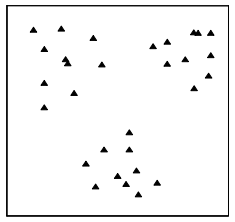
\includegraphics[width=4cm]{1.png}
		\label{fig:2a}
	}
	\end{minipage}
	\hfill
	\begin{minipage}[hbt]{4cm}
	\subfloat[initiale $k$ Punkte mit $k = 3$] {	
		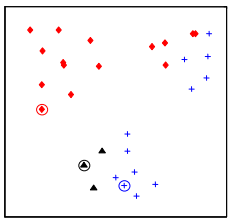
\includegraphics[width=4cm]{2.png}
		\label{fig:2b}
	}
	\end{minipage}
	\hfill	
	\begin{minipage}[hbt]{4cm}
	\subfloat[Iteration $2$] {	
		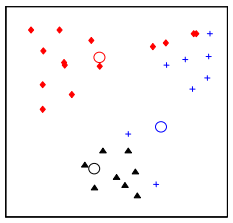
\includegraphics[width=4cm]{3.png}
		\label{fig:2c}
	}
	\end{minipage}
	\hfill
	\begin{minipage}[hbt]{6cm}
		\leftskip=2.5cm
		\subfloat[Iteration $3$] {
		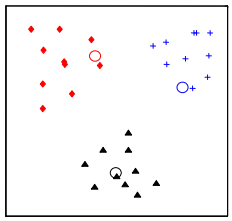
\includegraphics[width=4cm]{4.png}
		\label{fig:2d}
	}
	\end{minipage}
	\hfill
	\begin{minipage}[hbt]{6cm}
		\leftskip=1.3cm
		\subfloat[Clustering beendet] {		
		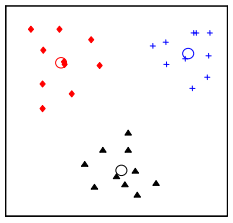
\includegraphics[width=4cm]{5.png}
		\label{fig:2e}
	}
	\end{minipage}
	\hfill
	\hfill\null
	\caption[Kantengraph]{
		Darstellung des K-Means-Clusterings an einem zweidimensionalen Beispieldatensatz (nach \citet{jain2010}) 
	}
	\label{fig:2}
\end{figure}

Nachteile des Lloyd-Algorithmus ergeben sich vor allem aus der zufälligen Wahl der initialen Clusterzentren. Hierdurch können einerseits im Laufe der Iterationen „leere“ Cluster entstehen, für die eine Kalkulation ihres Clusterzentrums nicht mehr möglich ist. Folglich können einmal entstandene „leere“ Cluster bei den folgenden Iterationen nicht mehr berücksichtigt werden. Andererseits werden vor allem lokale Optima bestimmt, die jedoch nicht unbedingt auch ein globales Optimum im Hinblick auf die Verteilung der Cluster über dem gesamten Datensatz darstellen \citep{Moris2013}.
\\

Die Ergebnisse des K-Means-Clusterings sind also maßgeblich von der initialen Wahl der $k$ Clusterzentren in Schritt~\ref{alg} des Algorithmus abhängig. Hierfür können $k$ Punkte gewählt werden, die von einander möglichst weit entfernt liegen. Ebenso können aus einer Stichprobe der Daten zunächst hierarchisch $k$ Cluster aufgebaut werden, aus denen dann jeweils ein Punkt als initiales Clusterzentrum zur Analyse des gesamten Datensatzes bestimmt wird. 
\\
\newpage
Die optimale Clusteranzahl $k$ lässt sich durch wiederholte Messungen ermitteln \citep{Moris2013}, insbesondere die Bestimmung des Clusterradius und -durchmessers sind hierfür geeignet. Der Clusterradius bezeichnet die maximale Distanz zwischen den Punkten des Clusters und seinem Clusterzentrum, der Clusterdurchmesser gibt die maximale Distanz zwischen zwei Punkten des Clusters an. Der durchschnittliche Radius bzw. Durchmesser eines Clusters verändert sich nur leicht beim Hinzufügen von weiteren Punkten, solange die Anzahl der zu erzeugenden Cluster der tatsächlichen Anzahl an Clustern im Datensatz entspricht oder höher liegt. Werden aber zwei Cluster zusammengefasst, die nicht zusammen passen, kommt es zu einem deutlichen Anstieg bei der Größe des Radius bzw. Durchmessers des Clusters. Eine effektive Vorgehensweise ist hierbei, für $ k $ Zweierpotenzen zu verwenden. Wurde dadurch ein passendes Intervall eingegrenzt, kann dieses Intervall ggf. durch weitere binäre Aufteilungen (binäre Suche) weiter angepasst werden, um so einen optimalen Wert für $ k $ zu ermitteln.

\section{Ward-Algorithmus} 

Dieser Algorithmus startet mit einem separaten Cluster für jeden Datenpunkt. Schrittweise werden die kleineren Cluster zu größeren  zusammengefasst, bis schließlich genau $ k $ Cluster gebildet wurden. Bei der Fusion der Cluster werden im Sinne eines Greedy-Algorithmus diejenigen Cluster zusammengefasst, welche die Varianz in einer Gruppe am wenigsten erhöhen \citep{Backh2008}. Problematisch bei diesem Clustering-Verfahren ist allerdings, dass der Algorithmus dazu tendiert, gleich große Cluster zu bilden \citep{Vos2004}, was jedoch bei realen Datensätzen eine eher ungewöhnliche Verteilung ist.  

\section{BFR-Algorithmus} 
\label{BFR}
Der Algorithmus nach \citet{Fayyad1998} (BFR-Algorithmus) wird  für Clusterdaten im mehrdimensionalen euklidischen Raum verwendet und eignet sich insbesondere für große Datenmengen, sogenannte Big Data. Voraussetzung für die Verwendung des Algorithmus ist allerdings, dass die Datenpunkte der Cluster in jeder Dimension eine Normalverteilung um die Clusterzentren herum besitzen. Dadurch wird eine runde/ellipsoide Clusterform um die Raumachsen herum impliziert. Der Mittelwert und die Standardabweichung dürfen sich in den verschiedenen Dimensionen unterscheiden, aber die Dimensionen müssen voneinander unabhängig sein. Abweichende Rotationen bezüglich der Raumachsen in den verschiedenen Dimensionen sind allerdings nicht zulässig.

\subsection{Initialisierung} 
Die initiale Auswahl einer optimalen Anzahl von $ k $ Punkten kann mit der bereits beim K-Means-Basisalgorithmus vorgestellten Methode (siehe Kapitel~\ref{Kap3}) erfolgen. Anschließend werden die Daten auf $ n $ verschiedene Stichproben zufällig aufgeteilt. Dies bietet den Vorteil, dass insbesondere bei Big Data nicht der gesamte Datensatz gleichzeitig in den Speicher eingelesen werden muss. Die Daten können in Fragmenten geladen werden, die relevanten Statistiken werden ermittelt und nur diese werden für die spätere Analyse des gesamten Datensatzes im Speicher belassen. Für diese relevanten Statistiken werden die folgenden drei Datenkategorien angelegt (siehe Abbildung~\ref{fig:BFR}):

\begin{itemize}
	\item \textbf{DS (Discard Set):} enthält die eigentlichen Cluster mit denjenigen Punkten, die nahe genug an einem der $ k $ Clusterzentren liegen, so dass sie einem Cluster sicher zugeordnet werden können (siehe Kapitel~\ref{Mahal}).
	
	\item \textbf{CS (Compressed Set):} enthält Gruppen von Datenpunkten, die zwar nahe bei einander liegen, aber keinem der zuvor festgelegten Clusterzentren zugeordnet werden konnten, da sich diese Punkte nicht nahe genug an einem der Clusterzentren befinden.
	
	\item \textbf{RS (Retained Set):} in dieser Kategorie werden isolierte Datenpunkte gesammelt, sie liegen weder nahe genug an den Clusterzentren des CS noch an denen des DS.
	
\end{itemize}

\subsection{Datenanalyse} 

Für jedes Cluster des DS bzw. CS werden folgende Werte berechnet (siehe Abbildung~\ref{fig:BFR}):

\begin{itemize}
	\item[\textbf{--}] $ N $ als Anzahl der Punkte des Clusters.
	\item[\textbf{--}] Der Vektor $ SUM $, dessen $ i $-tes Element jeweils der Summe der Koordinaten der $ i $-ten Dimension $ d $ von allen im Cluster enthaltenen Punkten entspricht. Dieser Vektor besitzt also die Länge $ d $.
	\item[\textbf{--}] Der Vektor $ SUMSQ $, dessen $ i $-tes Element jeweils die Summe der Koordinatenquadrate der $ i $-ten Dimension von allen im Cluster enthaltenen Punkten darstellt. Dieser Vektor besitzt ebenfalls die Länge $ d $.
\end{itemize}

Bei $ d $-dimensionalen Daten wird also jedes Cluster des DS und des CS durch $ 2d + 1 $ Werte repräsentiert. Ziel ist es ein Set der Daten zu erzeugen, in dem ihre Anzahl, ihr Clusterzentrum und ihre Standardabweichung für jede Dimension gespeichert ist. Die o.g. $ 2d + 1 $ Werte ermöglichen diese Metadaten:
\begin{itemize}
	\item[\textbf{--}] \textbf{Anzahl der Datenpunkte:} ist durch $ N $ bereits gespeichert.
	\item[\textbf{--}] \textbf{Clusterzentrum:} aufgrund der Normalverteilung in jeder Dimension, entsprechen die Koordinaten des Clusterzentrums den Mittelwerten der Datenpunktkoordinaten in jeder Dimension. Somit können die Koordinaten des Clusterzentrums durch die Elemente des SUM-Vektors für jede $ i $-te Dimension dargestellt werden durch:  \[\frac{SUM_{i}}{N} \]
	\item[\textbf{--}] \textbf{Standardabweichung:} durch die $ SUM $- und $ SUMSQ $-Vektoren lässt sich die Varianz $v$ in der $i$-ten Dimension wie folgt ermitteln:
	\[ v = \frac{SUMSQ_{i}}{N}-\left(\frac{SUM_{i}}{N}\right)^2 \] 
	Aufgrund der Normalverteilung der Daten kann hieraus auch die Standardabweichung $ s $ bestimmt werden, denn es gilt
	$s = \sqrt{v}$.
\end{itemize}


\begin{figure}[!htb]
	\centering
	\fbox{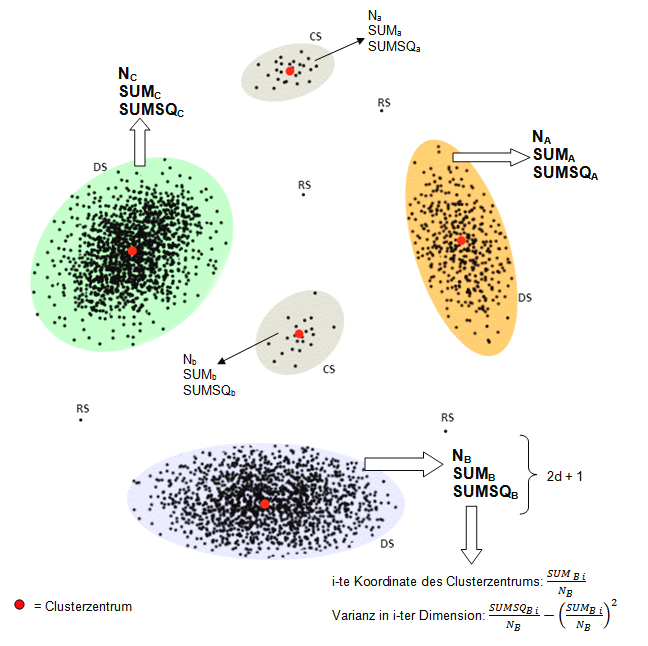
\includegraphics[width=15cm]{ClustersetsFinal.png}}
	\hfill\null
	\caption{Darstellung der Datenkategorien des BFR-Algorithmus und der aus ihnen ermittelten Werte.
	}
	\label{fig:BFR}
\end{figure}
\newpage
\noindent
\textbf{Aktualisierung der Metadaten:} \\
\\
\noindent
Die Punkte werden einzeln den Sets zugeordnet. Sobald ein Datenpunkt dem DS oder CS zugeordnet wurde, werden $ N $, $ SUM $ und $ SUMSQ $ für das entsprechende Cluster angepasst und der Punkt wird verworfen. Dadurch ist eine sehr einfache Aktualisierung des Clusterzentrums und der Standardabweichung möglich:
\begin{itemize}
	\item[\textbf{--}] Die Anzahl der Daten wird um $ 1 $ erhöht: 
	$ N + 1 $.
	\item[\textbf{--}] Die Koordinaten des Punktes werden zum $ SUM $-Vektor hinzuaddiert.
	\item[\textbf{--}] Die Quadrate der Koordinaten des Punktes werden zum $ SUMSQ $-Vektor hinzuaddiert. 
\end{itemize}	


Würden hier statt des $ SUM $-Vektors direkt die Koordianten des Clusterzentrums verwendet werden, so würde die Berechnung der Standardabweichung beim Hinzufügen eines neuen Punktes deutlich komplexer werden.
\\
\\
\noindent
\textbf{Zuordnung der Punkte zu den Datensets:}
\begin{enumerate}
	\item Datenpunkte, die nahe genug an einem Clusterzentrum liegen werden dem DS bzw. CS zugeordnet.
	\item Datenpunkte, die nicht nahe genug an einem der Clusterzentren liegen, werden mit den bislang vorhandenen Punkten im RS (aller vorherigen Stichproben) geclustert und falls möglich zu Compressed Sets zusammengefasst. Diejenigen Datenpunkte, die zu einem CS zusammengefasst wurden, werden aus dem RS entfernt. 
	\item Die so neu entstandenen CS werden mit den bereits vorhandenen CS abgeglichen und ggf. zu einem größeren CS zusammengefasst, falls sie nahe beieinander liegen. $ N $, $ SUM $ und $ SUMSQ $ werden beim zusammenführen der CS entsprechend aufsummiert.
\end{enumerate}	
	
Durch die schrittweise Verteilung der Datenpunkte auf DS, CS und RS bei jeder Stichprobe, erfolgt eine permanente Anpassung bzw. Korrektur der $ k $ Cluster, für die durch $ N $, $ SUM $ und $ SUMSQ $ die Koordinaten ihrer Clusterzenteren sowie ihre Standardabweichung in jeder Dimension gespeichert werden.
\\
\par
Nach Analyse aller Stichproben können alle verbliebenen CS und alle verbliebenen Datenpunkte des RS dem am nächsten liegenden Clusterzentrum zugewiesen werden. 
Ebenso besteht die Möglichkeit, diese Punkte als Ausreißer im Bezug auf das RS und Minicluster im Bezug auf das CS zu behandeln.

\subsection{Distanzmaß} \label{Mahal}

Um zu entscheiden, ob ein Datenpunkt nahe genug an einem der Clusterzentren des DS bzw. CS liegt, wird beim BFR-Algorithmus als Distanzmaß die Mahalanobis-Distanz verwendet. Die Mahalanobis-Distanz berücksichtigt im $ d $-dimensionalen Raum die Normalverteilung der Datenpunkte um das Clusterzentrum und damit die ellipsoide Form der Cluster. Bei Verwendung der euklidischen Distanz würde hingegen ein kreisförmiger Bereich um das Clusterzentrum berücksichtigt werden. Dadurch könnte ein Punkt durchaus außerhalb eines ellipsoiden Clusters liegen und würde dem Cluster dennoch zugeordnet werden. 
\\

Die Mahalanobis-Distanz bestimmt somit auch indirekt die Wahrscheinlichkeit eines Datenpunktes, einem bestimmten Cluster anzugehören und zwar in Abhängigkeit von der Normalverteilung um das Clusterzentrum. Mit den im DS bzw. CS gespeicherten Werten kann die Mahalanobis-Distanz für jeden Punkt wie folgt leicht berechnet werden.\\

%\noindent\hspace*{10mm}
\noindent
Seien die Koordinaten eines Clusterzentrums gegeben durch:
\[c = (c_{1}, c_{2}, ... , c_{d}) = \left(\frac{SUM_{1}}{N}, \frac{SUM_{2}}{N}, ... , \frac{SUM_{d}}{N} \right)\]
%\noindent\hspace*{10mm}
Und seien die Standardabweichungen des Clusterzentrums in jeder Dimension 
%\noindent\hspace*{10mm}
gegeben durch:
\begin{flalign*}
\sigma &= (\sigma_{1}, ... , \sigma_{d})\\
 &= \left(\left(\frac{SUMSQ_{1}}{N} - \left(\frac{SUM_{1}}{N}\right)^2 \right), ... ,
\left(\frac{SUMSQ_{d}}{N} - \left(\frac{SUM_{d}}{N}\right)^2 \right)\right)
\end{flalign*}
Für einen Punkt $ a $ mit den Koordinaten $ a = (a_{1}, a_{2}, ... , a_{d}) $ errechnet sich die normalisierte (euklidische) Distanz $ z $ in der Dimension $ i $ durch:
\[z_{i} = \frac{a_{i}-c_{i}}{\sigma_{i}}\]
\noindent
Die Mahalanobis-Distanz $ MD $ ergibt sich dann aus der Summe der quadrierten, normalisierten Distanzen jeder Dimension zu diesem Clusterzentrum:
\[MD = \sqrt{\sum_{i=1}^{d} z_{i}^2 }\]
\noindent
Durch Festlegung einer bestimmten Grenze ($ 1 $-, $ 2 $-, $ 3 $-fache Standardabweichung) kann entschieden werden, ob ein Punkt einem bestimmten Cluster zugeordnet wird.
Diese Grenze kann bestimmt werden, indem ein Punkt angenommen wird, der in jeder Dimension genau die einfache Standardabweichung vom Clusterzentrum entfernt liegt. Dann gilt: 
\[z_{i} = \frac{\sigma_{i}}{\sigma_{i}} = 1\]
Und somit:
\[MD = \sqrt{\sum_{i=1}^{d} 1^2 } = \sqrt{d}\]

Eine Grenze für die $ 2 $- bzw. $ 3 $-fache Standardabweichung wären somit $ 2\sqrt{d} $ bzw. $ 3\sqrt{d} $.
Im Grunde beschreibt die Mahalanobis-Distanz also die Korrelation zwischen einem Datenpunkt und dem Clusterzentrum, d.h. die Mahalanobis-Distanz nimmt zu, wenn die Korrelation abnimmt \citep{Backh2008}.
\\

Um zu bestimmen, ob zwei CS nahe genug beieinander liegen, um zusammengefasst zu werden, wird die Varianz beider CS-Subcluster kombiniert. Hierzu werden von beiden CS-Clustern $ N $, $ SUM $ und $ SUMSQ $ aufsummiert und aus diesen Werten die Varianz des neuen kombinierten Clusters bestimmt. Wenn die so ermittelte Varianz unterhalb einer festgelegten Grenze liegt, werden beide CS zusammengeführt.

\subsection{Kritische Betrachtung des BFR-Algorithmus}

Im Gegensatz zum K-Means-Basisalgorithmus arbeitet der BFR-Algorithmus nicht iterativ, sondern es werden multiple Lösungen für multiple Startpunkte generiert und im Laufe der Datenanalyse ggf. fusioniert \citep{bradley1998}. Der Datensatz muss also lediglich ein Mal durchlaufen werden. 
\\

Da für die analysierten Daten lediglich die Parameter $N$, $SUM$ und $SUMSQ$ gespeichert werden, ermöglicht der BFR-Algorithmus die Analyse großer Datensätze unter sparsamem Einsatz des verfügbaren Speicherplatzes. Allerdings ist es durch die Verwendung dieser wenigen Parameter nicht mehr möglich einzelne Datenpunkte aus den gewonnenen Statistiken abzurufen. Ebenso können Hintergrundrauschen und Ausreißer das Ergebnis des BFR-Algorithmus deutlich beeinflussen \citep{kumar}. Insbesondere kann sich bei großen, stark streuenden Datensätzen eine große Datenmenge im RS-Set ansammeln. Bei der Analyse von Big-Data-Datensätzen kann dies zu Problemen bezüglich des Speicherplatzbedarfes führen.
\\

Auch das strenge Kriterium der Normalverteilung um das Clusterzentrum und die damit verbundene ellipsoide Form der Cluster kann sich als problematisch erweisen. Wie \citet{kumar} ebenfalls kritisch anmerkt, ist dieses Kriterium bei realen Messdaten häufig nicht gegeben. Auch kann das Kriterium der ellipsoiden Clusterform durch überlappende bzw. fusionierte Cluster gestört werden.
\\

Insgesamt stellt der BFR-Algorithmus also eine gute Analysemethode für multivariante Big-Data-Datensätze dar, die das Kriterium der Normalverteilung um das Clusterzentrum herum erfüllen und eine möglichst geringe Streuung zwischen den Clustern aufweisen. 

\newpage
\section{Ausblick}

Neben den vorgestellten K-Means-Algorithmen finden sich in der Literatur zahlreiche Abwandlungen und Weiterentwicklungen der K-Means-Clusteringmethode \citep{Bagir2006,wu2008,Aletti2017}. Sie finden insbesondere im Bereich der Molekulargenetik und Proteinanalyse Anwendung. 
\\

Ein in den vergangenen Jahren stark wachsender Zweig der Molekulargenetik ist die Genexpressionsanalyse, insbesondere im Bereich der Tumorforschung. Hierbei wird zeitgleich die Aktivität von in der Regel mehreren tausend Genen gemessen. Um Veränderungen bezüglich einer Erkrankung oder der Effizienz einer Therapie feststellen zu können, werden dazu die Genaktivitäten im kranken bzw. behandelten Gewebe im Vergleich zum gesunden gleichartigen Gewebe des selben Individuums betrachtet. Auf diese Weise lässt sich eine verstärkte Aktivierung oder Hemmung bestimmter Gene im krankhaft veränderten oder behandelten Gewebe detektieren. 
\\

Mithilfe des K-Means-Clusterings und auch anderer Clusteringverfahren können nun Gruppen von Genen identifiziert werden, welche ähnliche Aktivitätsmuster zeigen (siehe Abbildung~\ref{hma} und~\ref{hmb}). Hierbei können Gene, die sich im gleichen Cluster befinden, die also ein ähnliches Aktivitätsmuster aufweisen, auf die Aktivierung oder Hemmung bestimmter Stoffwechselwege hindeuten. Die so identifizierten Stoffwechselwege können Ansatzpunkte für neue Therapien der untersuchten Erkrankung darstellen. 


\begin{figure}[!htb]
	\centering
	\null\hfill
	\fbox{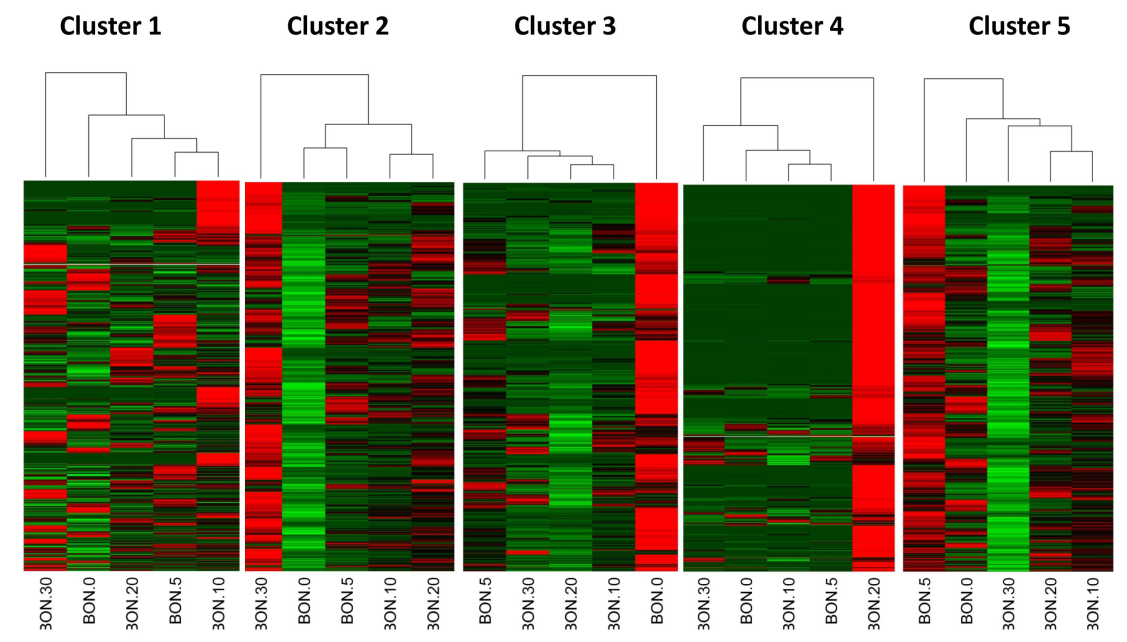
\includegraphics[width=15 cm]{Sarropou.png}}
	\caption{
		Expressionsprofile verschiedener mittels K-Means-Clustering gruppierter Gene aus verschiedenen Larvenstadien des Atlantik-Thunfischs (rot: verstärkte Genaktivität, grün: reduzierte Genaktivität) \citep{Sarrop2014}.
	}
	\label{hma}
\end{figure}

\begin{figure}[!htb]
	\centering
	\null\hfill
	\fbox{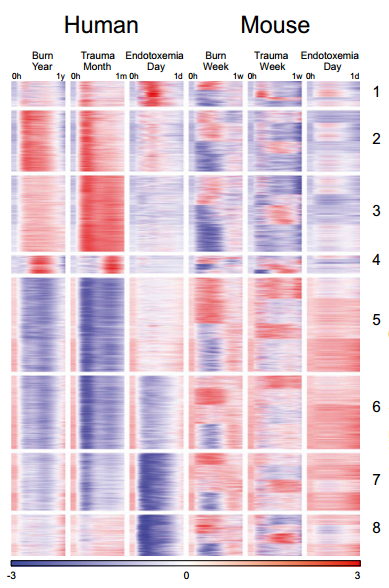
\includegraphics[width=13 cm]{Seok.png}}
	\caption{
		K-Means-Clustering von 4918 entzündungsassoziierten Genen bei Mensch und Maus \citep{Seok2013}. Die Messungen erfolgten zu verschiedenen Zeitpunkten im Anschluss an bestimmte entzündungsinduzierende Ereignisse. Rote Bereiche entsprechen verstärkt exprimierten Genen, blaue Bereiche zeigen Gene mit reduzierter Genaktivität an.
	}
	\label{hmb}
\end{figure}
\clearpage

%------------------------------------------------
% Literaturverzeichnis
%------------------------------------------------

\newpage
\bibliographystyle{abbrvnat-ger}
\bibliography{kmeans}
\addcontentsline{toc}{section}{\bibname}


\end{document}
